%
% File acl2019.tex
%
%% Based on the style files for ACL 2018, NAACL 2018/19, which were
%% Based on the style files for ACL-2015, with some improvements
%%  taken from the NAACL-2016 style
%% Based on the style files for ACL-2014, which were, in turn,
%% based on ACL-2013, ACL-2012, ACL-2011, ACL-2010, ACL-IJCNLP-2009,
%% EACL-2009, IJCNLP-2008...
%% Based on the style files for EACL 2006 by
%%e.agirre@ehu.es or Sergi.Balari@uab.es
%% and that of ACL 08 by Joakim Nivre and Noah Smith
% chktex-file 19
% chktex-file 13
% chktex-file 24
% chktex-file 8
% chktex-file 44
% chktex-file 45
% chktex-file 46

\documentclass[11pt,a4paper]{article}
\usepackage[hyperref]{acl2019}
\usepackage{times}
\usepackage{latexsym}
\usepackage{url}

\usepackage{placeins}

\usepackage[utf8]{inputenc}
\usepackage[russian,english]{babel}

\usepackage{listings}
\usepackage{multirow}
\lstset{basicstyle=\ttfamily, keywordstyle=\rmfamily\bfseries}

\usepackage[final]{graphicx}
\usepackage{amsmath,amssymb}
\usepackage{algorithm}
\usepackage{pgfplots}
\usepackage{enumerate}
\usepackage{url}
\usepackage[outdir=./]{epstopdf}
\usepackage{flushend}
\usepackage[most]{tcolorbox}
\setlength{\fboxsep}{2pt}
\usepackage[T1]{fontenc}
\usepackage[utf8]{inputenc}
\usepackage[russian,english]{babel}


%\aclfinalcopy % Uncomment this line for the final submission
%\def\aclpaperid{***} %  Enter the acl Paper ID here

%\setlength\titlebox{5cm}
% You can expand the titlebox if you need extra space
% to show all the authors. Please do not make the titlebox
% smaller than 5cm (the original size); we will check this
% in the camera-ready version and ask you to change it back.

\newcommand\BibTeX{B\textsc{ib}\TeX}

\title{Automatic WordNet Construction using Cross-lingual Embeddings}

\author{Denis Gordeev, Alexey Rey, Dmitry Shagarov
	First Author \\
  Affiliation / Address line 1 \\
  Affiliation / Address line 2 \\
  Affiliation / Address line 3 \\
  \texttt{email@domain} \\\And
  Second Author \\
  Affiliation / Address line 1 \\
  Affiliation / Address line 2 \\
  Affiliation / Address line 3 \\
  \texttt{email@domain} \\}

\date{}

\begin{document}
\maketitle
\begin{abstract}
Low-resource languages often lack structured text representations (taxonomies, ontologies and lexical databases). In this paper we propose a method for constructing WordNets from Princeton WordNet without translation engines or parallel corpora. The proposed method uses cross-lingual word embeddings and outperforms translation-based techniques in F1-score. We also publish automatically constructed general truncated WordNets and collocation WordNets for 44 languages (including non-European ones) \footnote{link removed to stay anonymous for the review process}.
\end{abstract}

\section{Introduction}
%ворднеты делали
%рассказать про русские ворднеты
%упомянуть другие ворднеты
%и про ходака

There are numerous structured information representations containing texts as titles, descriptions or definitions: e.g.\ ontologies, taxonomies, and lexical databases. Among such databases we can highlight WordNet \cite{wordnet}. WordNet is a lexical database covering various types of relations between words: both semantical and lexical. Semantic concepts called synsets are connected in accordance to the semantical and lexical relations between them. The database has found a very broad usage for many natural language processing and machine learning applications \cite{kutuzovgraphwordnet,mao-semeval}.
There have been many attempts by researchers to automatically convert WordNet from English into other languages. Most attempts were focused on using machine translation engines, extensive bilingual dictionaries or parallel corpora~\cite{Khodak2017,NEALE18.1030} which are often lacking for low-resource languages.

In this paper we propose a method for constructing WordNets using cross-lingual embeddings. Unlike previous attempts our method does not require translation engines or parallel corpora. There have been already works using word embeddings for extending existing WordNets \cite{sand2017wordnet,tarouti} in monolingual settings. However, these methods could not be used for creating a WordNet for another language from scratch.

Word embeddings proved to be a powerful tool for dense text representations after papers by Bengio~\cite{bengio} and Mikolov~\cite{mikolov-representations-2013}. However, first word vector representation models were monolingual only. Soon researchers proposed cross-lingual word embedding models~\cite{mikolov-parallel}. There followed several improvements to the original model. In \citeyear{artetxe2016learning} Arxetxe et al. found that Procrustes refinement gets better results than the original linear transformation method by Mikolov. Besides most earlier methods suffered from the "hubness problem" where some words (especially low frequency ones) appear in the top neighbour lists of many other words.

Alexis Conneau et al. in (\citeyear{muse}) offered a method called cross-domain similarity local scaling (CSLS) to overcome this problem. They reached 81.7\% accuracy for English-Spanish and 83.7\% for Spanish-English pairs for top-1500 source queries in a completely unsupervised mode. For English-Russian and Russian-English their results are not as high and they achieved accuracy of 51.7\% and 63.7\% respectively. Their FastText embeddings were trained on Wikipedia datasets for each language respectively. They have published aligned embeddings for 30 languages \footnote{https://github.com/facebookresearch/MUSE}. Joulin et al. in (\citeyear{joulin2018loss}) found that convex relaxation of the CSLS loss improves the quality of bilingual word alignment. They have also published aligned FastText vectors with vocabularies of more than 2 million words and phrases \footnote{https://fasttext.cc/docs/en/aligned-vectors.html} (Fig. \ref*{wordvectors}).

Many researchers have used a similar method for detecting new hypernyms-hyponyms relations beyond WordNet for English. The work by \cite{sanchez2017well} has provided an overview of such methods. Such models may achieve up to 81.2 \%accuracy after removing noise samples.


\section{Cross-lingual embeddings}

MUSE is based on the work by Conneau et al.~\cite{muse}. It consists of two algorithms. The first one which is used only in unsupervised scenarios is a pair of adversarial neural networks. The first neural network is trained to predict from which distribution $\{X, Y\}$ embeddings come. The second neural networks is trained to modify embeddings $X$ multiplying it by matrix $W$ to prevent the first neural network from making accurate discriminations. Thus, at the end of the training we get a matrix $WX$ which is aligned with matrix $Y$.

\begin{figure}
	
	\centering
	\small
	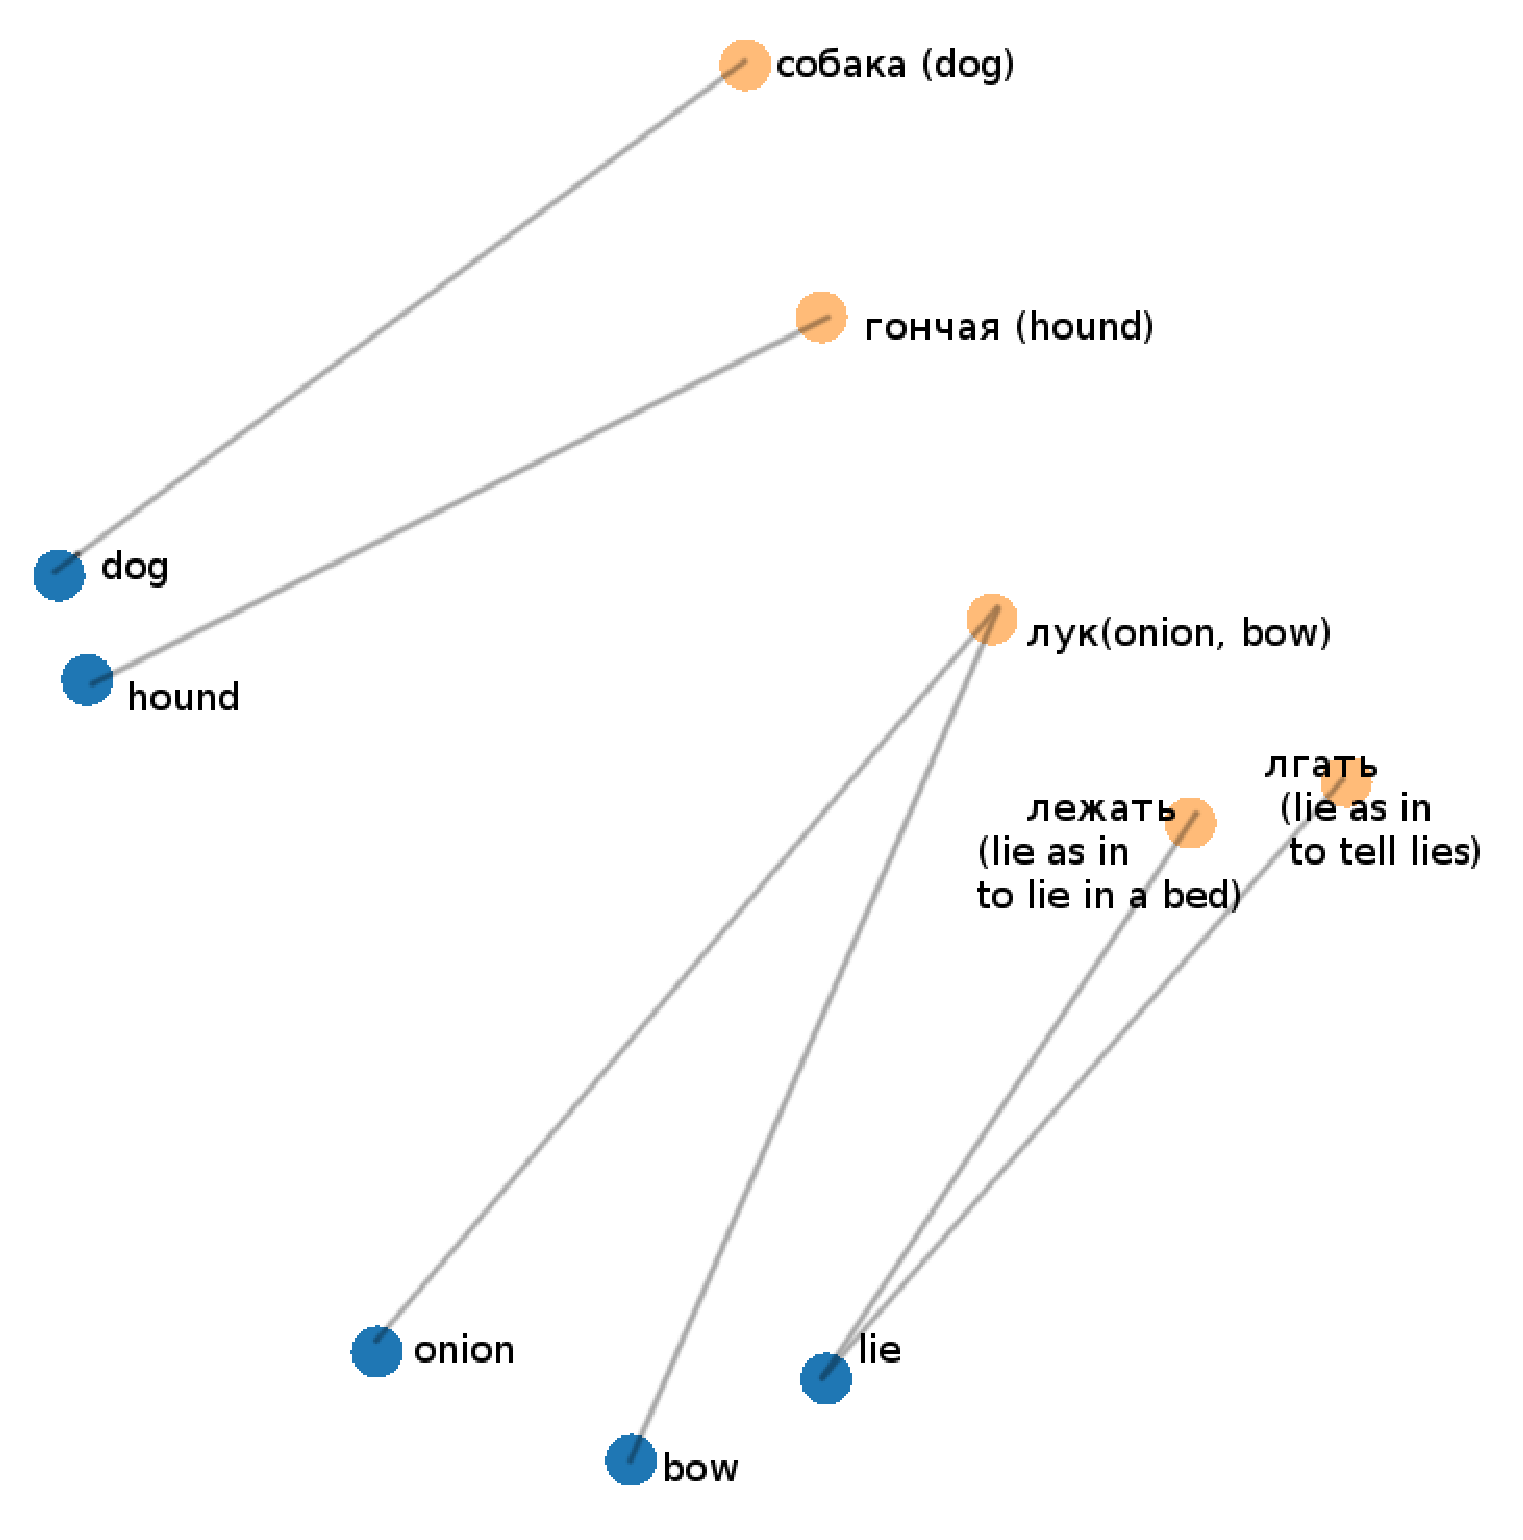
\includegraphics[scale=0.3]{wordvectors}\\
	
	\caption{PCA visualization of aligned word embeddings for Russian and English}
	\label{wordvectors}
\end{figure}


The second method is supervised and the aim is to find a linear mapping $W$ between embedding spaces $X$ and $Y$ which can be solved using Orthogonal Procrustes problem:

$$ W^* = argmin_W ||WX - Y||_F = UV^T$$

where $UV^T$ is derived using singular value decomposition SVD$(YX^T) = U \Sigma V^T$.
This method is used iteratively with the default number of iterations in MUSE equal to 5. As Søgaard, Ruder and Vulić state Procrustes refinement relies on frequent word pairs serving as reliable anchors.

Conneau et al.\ also apply cross-domain similarity local scaling to lessen the extent of hubness problem which cross-lingual embeddings are prone to~\cite{dinu}. It uses cosine similarity between a source embedding vector $x$ and $k$ target nearest embeddings $\mathcal{N}$ (the default $k$ in MUSE is 10) to generate a dictionary.
\begin{align*}
sim(x, y) = \dfrac{1}{k}\sum_{i=1}^K\cos(x, {\mathcal{N}_X}_i);\\
\mathcal{N}_X \in Y=\{y_1,...,y_n\} 
\end{align*}
\small
$$CSLS(x,y) = 2\cos(x,y) - sim_{source}(x, y)  - sim_{target}(y, x)$$
\normalsize

Vecmap~\cite{vecmap} is close in its idea to the Procrustes refinement, it computes SVD-factorization SVD$(YX^T) = U\Sigma V^T$ and replaces $X$ and $Y$ with new matrices $X' = U$ and $Y' = V$. The authors also propose normalization and whitening (sphering) transformation. After applying whitening new matrices are equal to:
$X' = {({X^T}X)}^{-\tfrac{1}{2}}$ and $Y' = {({Y^T}Y)}^{-\tfrac{1}{2}}$

Jawanpuria et al.~\cite{jawanpuria} propose a method which is, likewise, based on SVD-factorization but in smooth Riemannian manifolds instead of Euclidean space.

Joulin et al. in (\citeyear{joulin2018loss}) introduced a reformulation of CSLS that can be generalized to convex functions (Relaxed CSLS loss). Due to the orthogonality constraint on $W$ and FastText vectors being $\ell_2$-normalized $\cos(Wx, y) = x^T W^Ty$ and $|| y - {W_X}_i ||^2_2 = 2 - 2x^TW^Ty$. The problem can be reformulated to find the $k$ elements of $Y$ which have the largest dot product with ${W_X}_i$. Thus, RCSLS can be written down as:

	\begin{align*}
	\underset{W \in  \mathcal O_d}{min} \dfrac{1}{n}\sum_{i=1}^{n} - 2x^T_iW^Ty_i \\
	+ \dfrac{1}{k} \sum_{y_j \in \mathcal{N}_Y({W_X}_i)}^{ } x_i^T W^Ty_j \\
	+ \dfrac{1}{k} \sum_{{W_X}_j \in \mathcal{N}_X(y_i)}^{ } x_j^T W^Ty_i
	\end{align*}

Thus, RCSLS can be solved using manifold optimization tools \cite{boumal2014manopt}.
\section{Proposed method}
\begin{figure}
	
	\centering
	\small
	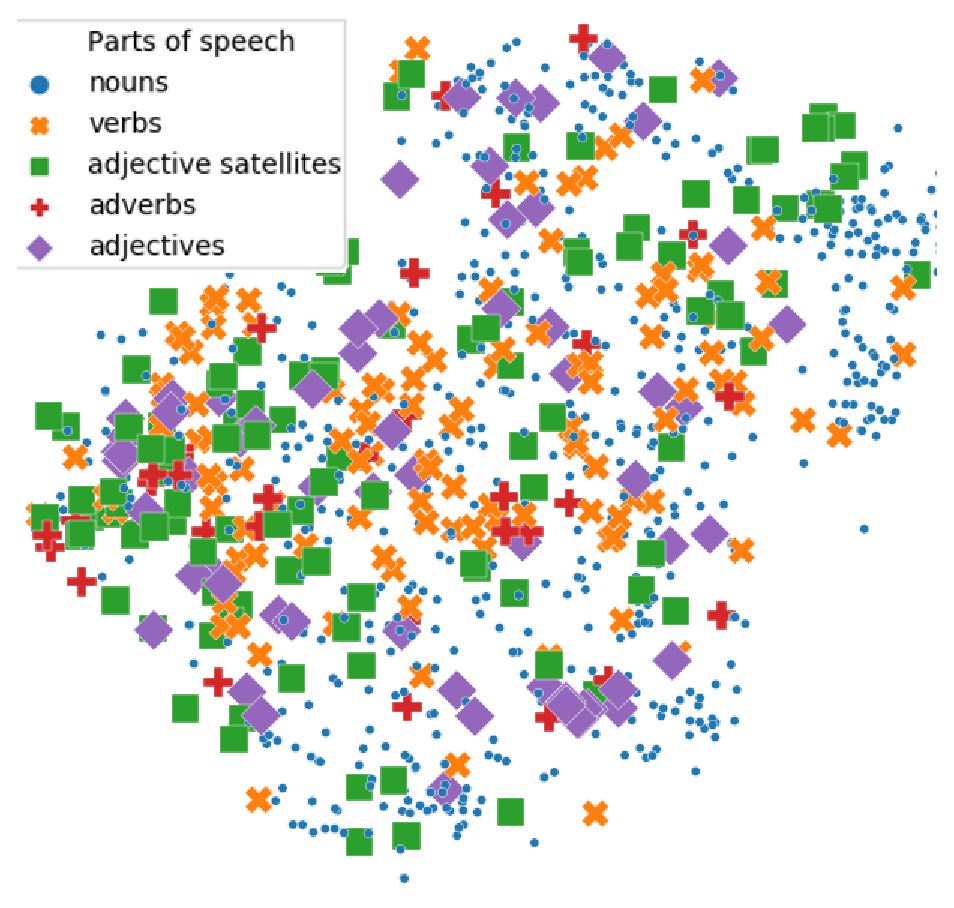
\includegraphics[scale=0.5]{wordnet-pos3}\\
	
	\caption{t-SNE visualisation of WordNet synset SIF-embeddings}
	\label{wordnet-pos}
\end{figure}
We reformulated the problem of synset finding as a binary classification problem. The task is to predict for the given (synset, lemma) pair whether they are related or not. As training/validation data we used English Princeton WordNet \cite{wordnet} provided by the NLTK package~\cite{nltk}. It contains 117'659 synsets. As positive examples we use (lemma, synset) pairs. As negative examples lemmas from other synsets with the same root are used (chicken.n.01 vs. chicken.n.02). We also added some random words because of scarcity of negative examples. There were also attempts at augmenting training data with synsets from from other languages besides English using the Open Multilingual WordNet \cite{Bond2012, bond-wordnet}. Unfortunately, only three models from the Open Multilingual WordNet contain 100\% of core Princeton WordNet word senses (5000 most popular synsets): the Finnish, the Chinese and the Croatian. In our experiments we used only Finnish Open WordNet because it is 100\% full and allows to avoid implicit bias towards Indo-European languages used for testing.

	\begin{table}[!htbp]
	\small
	\caption{Training data for chicken.n.01 (the flesh of a chicken used for food)}
	\label{wordnet-training-data}		
	\centering
	\begin{tabular}{|l|l|l|}
		\hline
		Word & Synset & Target
		\\
		\hline
		chicken & chicken.n.01 & 1
		\\
		poulet & chicken.n.01 & 1
		\\
		yellow & chicken.n.01 & 0
		\\
		chickenhearted & chicken.n.01 & 0
		\\
		visible & chicken.n.01 & 0
		\\
		\hline
	\end{tabular}
	
\end{table}

Synset embeddings were calculated using averaged synset lemma embedding and the definition embedding. As lemma and definitions are in English, MUSE or RCSLS pretrained English models were employed for embeddings generation. We used averaging weights 0.2 for the lemma and 0.8 for the definition (best at the validation dataset). SIF (smooth inverse frequency) and TF-IDF (term frequency–inverse document frequency) averaging schemes were employed for definition embeddings. SIF \cite{Arora2017} embeddings use pre-trained word vectors. For each sentence $s$ this model first creates a vectorized averaged representation $V_s$.

$$V_s = \dfrac{1}{|s|}\sum_{w \in s} \frac{a}{a + p(w)}V_w$$
where $V_w$ is the word unigram probability and $a$ is a scalar (set to 1e-3 by default).
After that all sentence embeddings are grouped into a matrix where $u$ is its first singular vector. The final sentence embedding is computed using this singular vector $u$.
$$V_s = V_s - uu^TV_s$$


For each lemma we used its embedding from the corresponding cross-lingual pre-trained model (\cite{muse} or \cite{joulin2018loss}) for the language.

Each synset embedding vector was augmented with a one-hot vector representing its part of speech and the synset number from the Princeton WordNet, empirically it was found that it provides a tiny boost to the final score.

Predicting synset relations is not a trivial task even in a monolingual setting. A simple linear model is unlikely to help in this case as we failed to get any meaningful cluster representation for synsets using t-SNE (t-Distributed Stochastic Neighbor Embedding) \cite{tsne} (Fig. \ref{wordnet-pos}). Moreover, there is not much training data and models are prone to overfitting in such circumstances. Thus, we introduced an ensemble of 4 LightGBM-models (Gradient Boosting Machine) \cite{lgbm} and 4 dense 3-layered fully-connected neural networks with dropout as regularization \cite{dropout} (Fig. \ref{keras_model}). LightGBM is an efficient, fast and easy to use Gradient Boosting model \cite{natekin2013gradient}.

In the neural network ReLU's (rectified linear units) were used for activations of hidden fully-connected layers ($f(x) = max(0, x)$). Sigmoid activation was used for the output layer ($f(x) = \frac{e^x}{e^x + 1}$). Dropout rates were set as (0.2, 0.2, 0.1). As the loss function we used binary cross validation which can be derived from cross validation:
\begin{align*}
 CE = -\sum_{i}^{C}y_{i} log (\hat{y}_{i})
\end{align*}
where $y$ are true and $\hat{y}$ are predicted labels.
For the binary case cross validation transforms into:
\begin{align*}
CE = -\sum_{i}^{2}y_{i} log (\hat{y}_{i}) \\
y_2 = 1 - y_1; \hat{y}_2 = 1 - \hat{y}_1 \\
CE = - (y_1log(\hat{y}_1) + (1 - y)log(1 - \hat{y}_1))
\end{align*}

All models prediction probabilities were averaged. After that classes were inferred using the threshold computed on the validation set. A more sophisticated ensemble approach might have improved results, but voting and individual model weighting schemes showed worse results in our case.

\begin{figure}[!htbp]
	
	\centering
	\small
	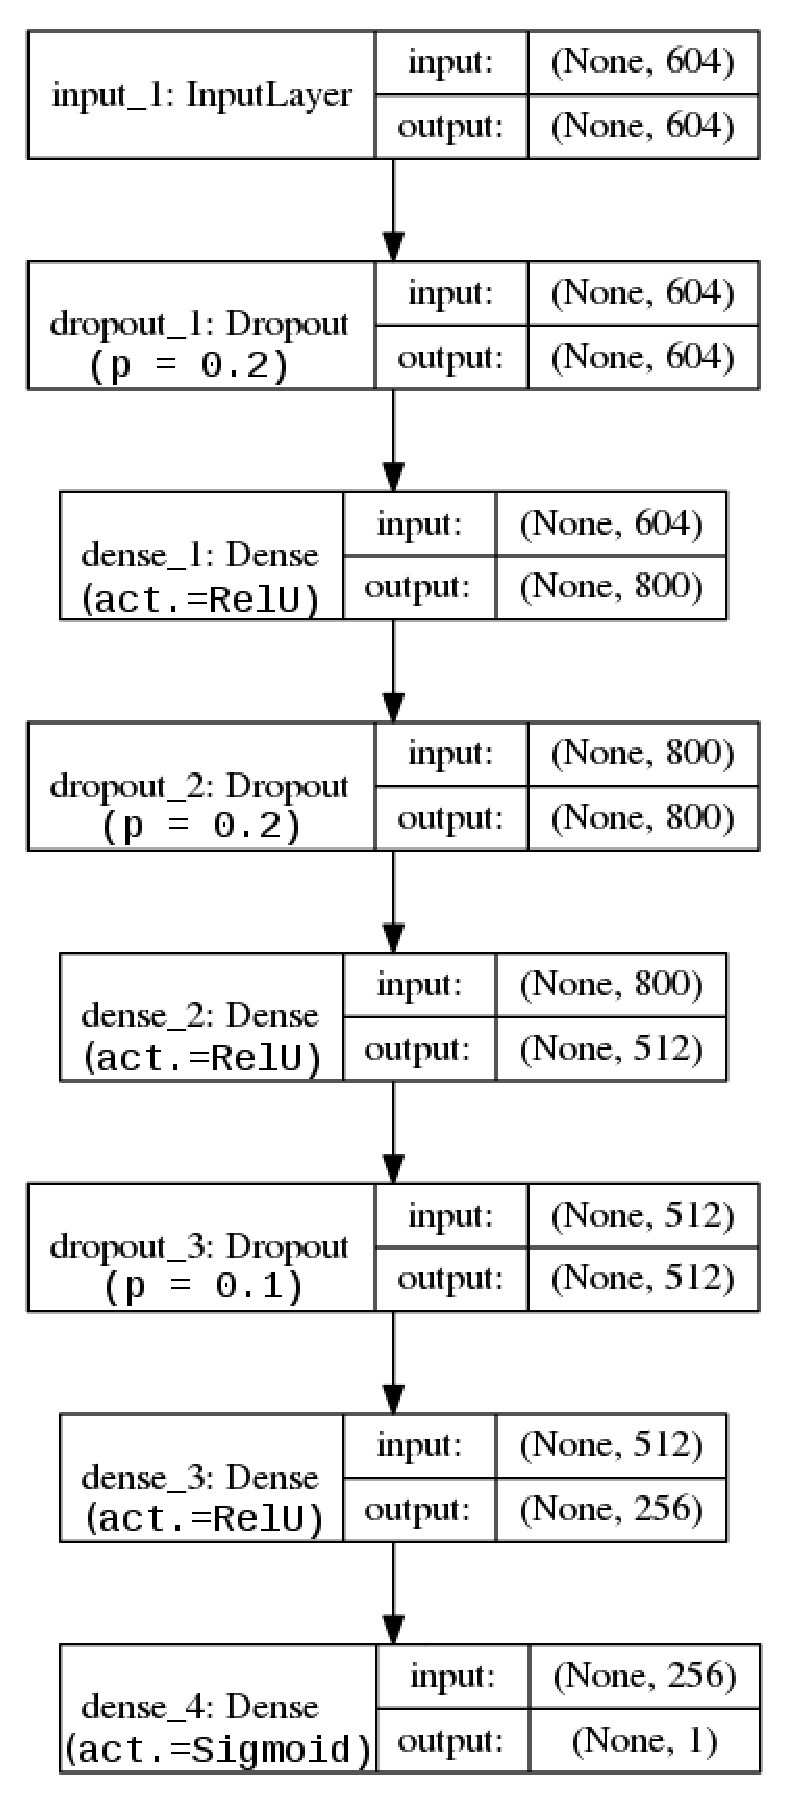
\includegraphics[scale=0.4]{keras_model2}\\
	
	\caption{Keras model}
	\label{keras_model}
\end{figure}

In our case parameters fine-tuning of the model classification threshold (e.g. the threshold to distinguish between two classes was not 0.5 but 0.42) using half of test data of the target language for validation (and removing it from the final test dataset) not only did not bring any benefit to the final score, but even decreased it significantly (about 3 F1-score points).

We also attempted to fine tune input data using PCA (principal component analysis) and UMAP (Uniform Manifold Approximation and Projection) \cite{umap} but it did not provide any gains, and brought about worse results.

For testing there were used two manually annotated datasets provided in the paper \cite{Khodak2017} for Russian and French languages respectively. Each dataset consists of 600 target language words from three parts of speech (nouns, verbs and adjectives). Each word has some true senses (synsets) and false ones (Table \ref{wordnet-test-data}). The original test procedure did not penalize models if some synsets were absent from the model and could not be predicted. In our case the RCSLS-model has the full coverage of the dataset, thus we were able to give predictions even for the rarest synsets.

\begin{table*}[!htbp]
	\small
	\caption{Test data by \cite{Khodak2017}}
	\label{wordnet-test-data}		
	\centering
	\begin{tabular}{l l l l}
		\hline
		Word & Target &  Synset & Definition \\ \hline
		\multirow{2}{*}{\begin{otherlanguage*}{russian}адрес \end{otherlanguage*}}
		& \multicolumn{1}{l}{1} & \multicolumn{1}{l}{address.n.01} & \multicolumn{1}{l}{(computer science) the code that identifies where a piece of information is stored} \\
		& \multicolumn{1}{l}{0} & \multicolumn{1}{l}{address.n.03} & \multicolumn{1}{l}{the act of delivering a formal spoken communication to an audience} \\
		\hline
		\multirow{2}{*}{aise}
		& \multicolumn{1}{l}{1} & \multicolumn{1}{l}{comfortable.a.01} & \multicolumn{1}{l}{providing or experiencing physical well-being or relief} \\
		& \multicolumn{1}{l}{0} & \multicolumn{1}{l}{comfortable.s.03} & \multicolumn{1}{l}{more than adequate; Example 1: the home team had a comfortable lead} \\
		\hline
	\end{tabular}
	
\end{table*}


\section{WordNet construction}
In line with previous works \cite{Vossen1998,tufis2006romanian} we extend an existing WordNet and match words from the target language to existing Princeton WordNet synsets. For this we use our ensemble model: for every word we predict its synsets.

Despite being easy to train, WordNet construction imposes significant computational problems in our case because we need to compare each word from the vocabulary with every possible synset. Luckily matrix calculus and modern machine-learning frameworks allow us to predict all synsets for several words in a single batch. However, to ease computation requirements we used several heuristics. 1) removed strings with punctuation besides the underscore symbol. 2) identified language using \cite{Joulin2016} for each string (FastText embeddings are noisy and contain a lot of samples from other languages).  All computations were vectorized. Ensemble methods also are easy to parallelize using the multiprocessing realization in Python and using bufferized numpy-arrays allows to increase the batch size and avoid copying data \cite{gorelick2014high}.

aaaaaaaaaaaaaaa

aaaaaaaaaaaaaaa

aaaaaaaaaaaaaaa

aaaaaaaaaaaaaaa

aaaaaaaaaaaaaaa

Candidate synsets were preselected using a simple model with a low threshold (0.2). However, we still had to limit the size of our WordNets. That is why we publish automated WordNets for all collocations and most common 10000 lemmas for 44 languages. To increase the quality of the generated models it was decided to sacrifice recall for the sake of precision and we increased the model confidence threshold to 0.6.

\section{Multiword Expressions}
\begin{figure}
	
	\centering
	\small
	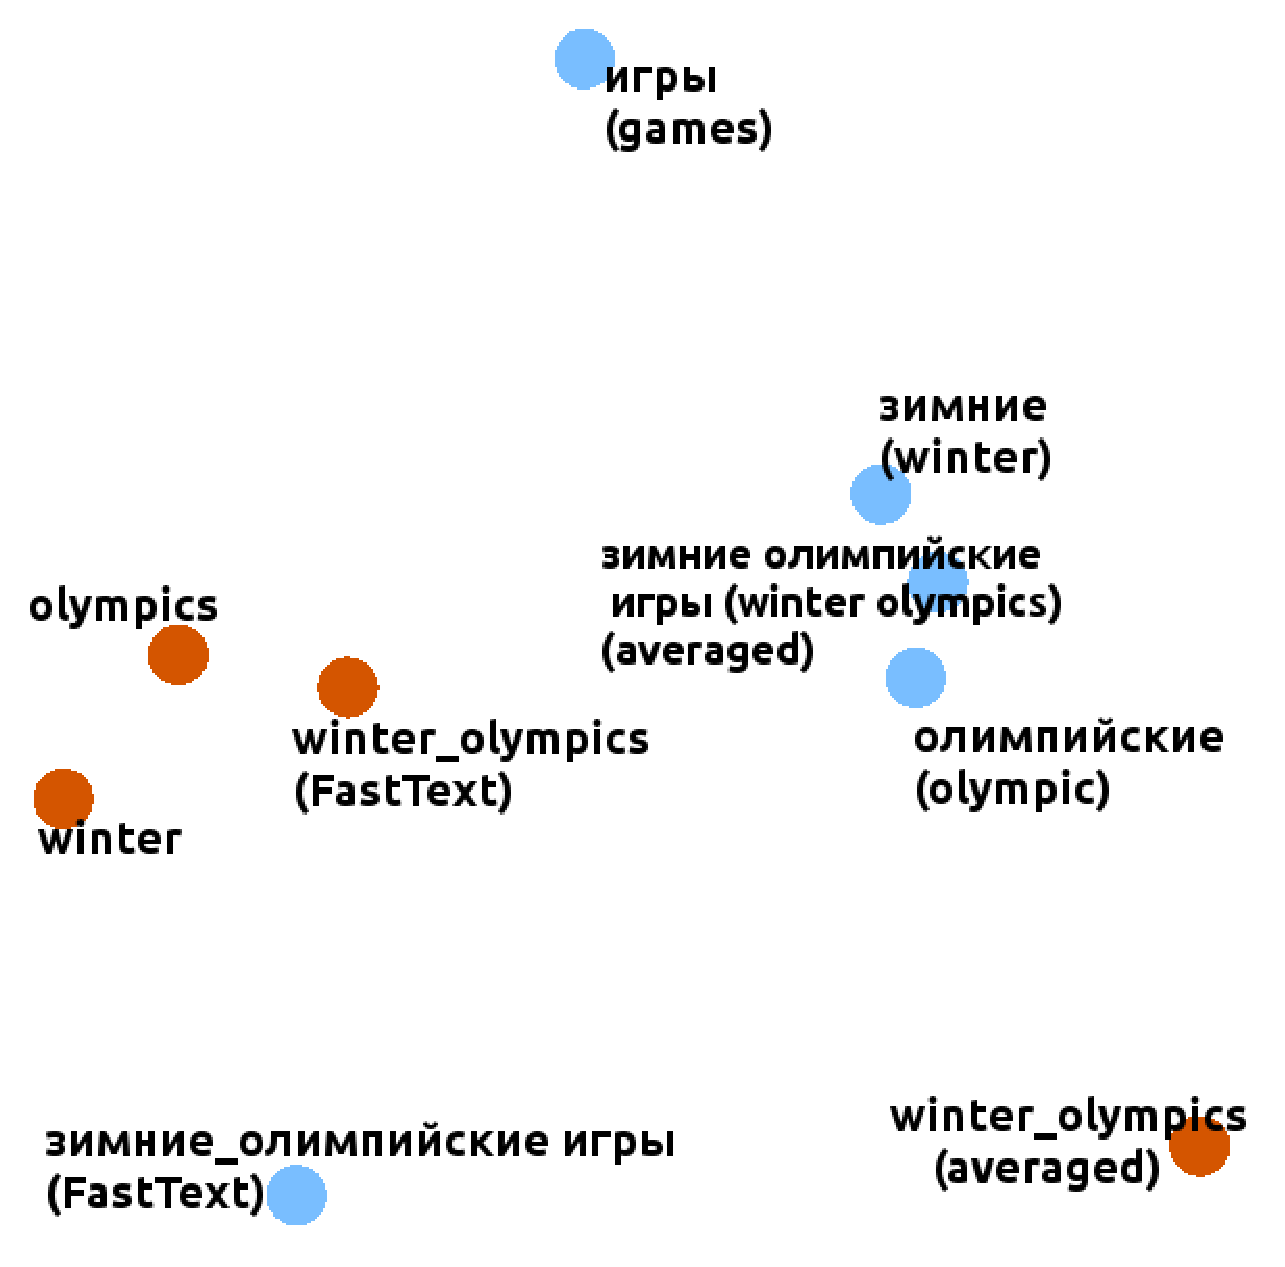
\includegraphics[scale=0.3]{mwe}\\
	
	\caption{t-SNE visualisation of averaged and FastText induced embeddings for MWE}
	\label{mwe}
\end{figure}

\section{WordNet Generation Pipeline}
\begin{figure}
	
	\centering
	\small
	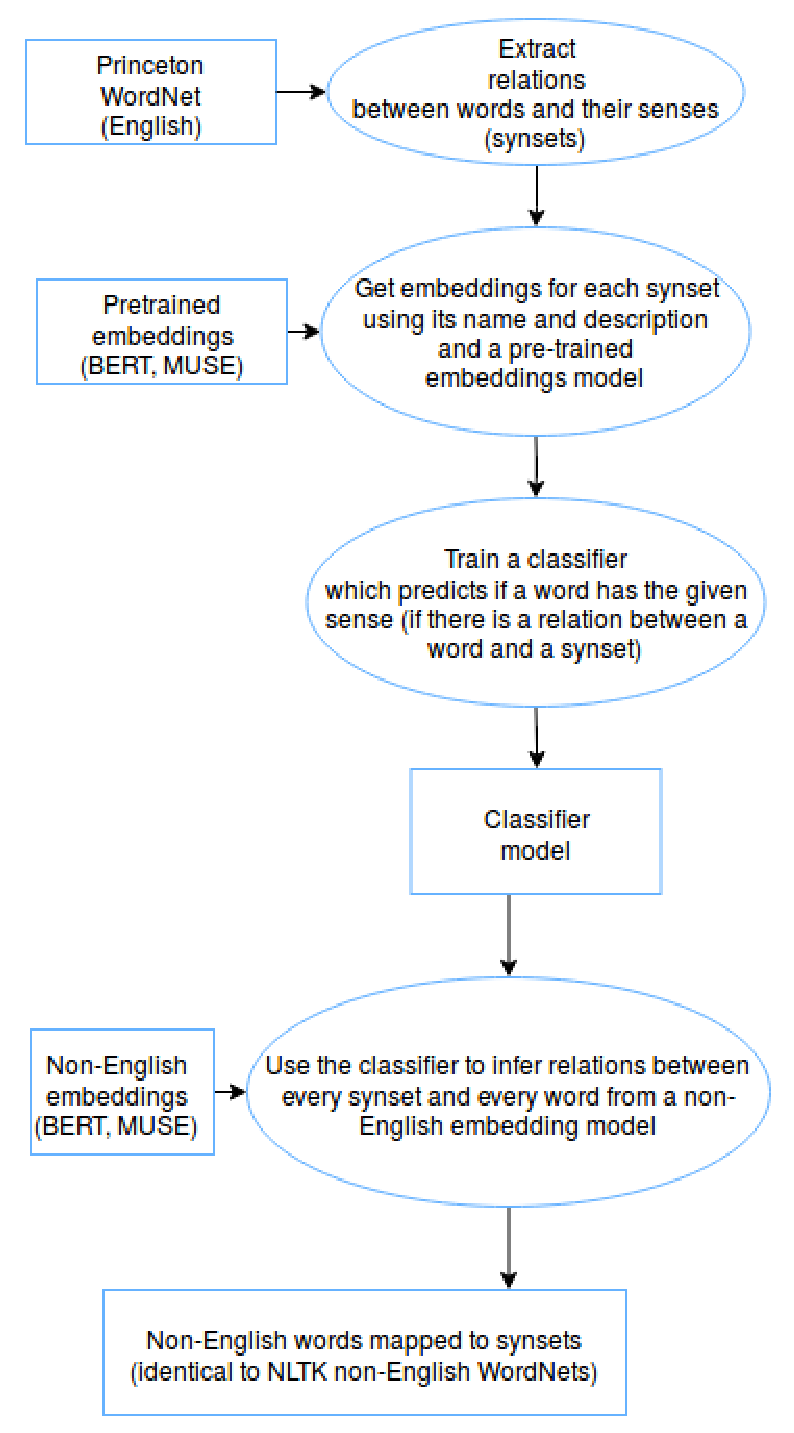
\includegraphics[scale=0.6]{pipeline}\\
	
	\caption{The pipeline showing WordNet generation using cross-lingual embeddings}
	\label{pipeline}
\end{figure}


We generated not only truncated WordNets but also WordNets for multiword expressions. Multiword expressions (MWE) are notoriously difficult to process and to model \cite{sag2002multiword}. A typical phrasing scheme used by Mikolov in Word2Vec (\citeyear{mikolov-representations-2013}) is a very simple	and rather efficient way to take phrase context into consideration and not just consider it as an average of its constituents \ref{mwe}.
$$score(w_i, w_j) = \frac{count(w_iw_j) - \delta}{count(w_i) * count(w_j)}$$

Other metrics such as PMI \cite{bouma2009normalized} or a special model for identifying MWE using a corpus like PARSEME \cite{savary2018parseme} might have been preferable. Yet in this work we were constrained by the multi-word expression scheme used in pretrained embeddings.
\begin{table}[!htbp]
	\small
	\caption{MWE examples for the aligned English RCSLS embeddings}
	\label{mwe-wiki}		
	\centering
	\begin{tabular}{|l|}
		\hline
		nearest\_city \\
		fiscal\_code \\
		architectural\_style \\
		population\_metro \\
		winners\_share \\
		third\_team \\
		people\_from\_new\_orleans \\
		parent\_agency \\
		\hline
	\end{tabular}
\end{table}

Another problem with FastText MWE is that the model is trained using the Wikipedia corpora. This leads to many artifact multi-word expressions corresponding to Wikipedia categories (Fig \ref{mwe-wiki}). Besides some synsets tend to be too general or of a wrong part of speech (Fig. \ref{mwe-results}). Still we decided to publish WordNet for this collocations as many of them are still relevant and correspond to multi-part verbs and real collocations (e.g. 'take notes', 'take away'). It also highlights the importance of another approach for MWE in word embedding models. Also some language embeddings do no contain any collocations (e.g. Korean).
\begin{table}[tp]
	\small
	\caption{Synset matching for MWE}
	\label{mwe-results}
	\centering
	\begin{tabular}{l l}
		\hline
		MWE & Synsets
		\\
		\hline
		\multirow{3}{*}{\shortstack[l]{\\ \begin{otherlanguage*}{russian}Тоталитарная секта \end{otherlanguage*}  \\ (totalitarian cult) (Russian)}}
		& \multicolumn{1}{l}{terrorization.n.02} \\
		& \multicolumn{1}{l}{cult.n.04} \\
		& \multicolumn{1}{l}{\shortstack{revolutionary\_organization\_\\ 17 november.n.01}} \\
		\hline
		\multirow{2}{*}{zweiter weltkrieg (German)}
		& \multicolumn{1}{l}{nazify.v.01} \\
		& \multicolumn{1}{l}{blitzkrieg.v.01} \\ \hline
		\multirow{2}{*}{\shortstack{gospodarska regija \\ (economic region) (Croatian)}}
		& \multicolumn{1}{l}{economic\_geography.n.01} \\
		& \multicolumn{1}{l}{zone.v.01} \\ \hline

	\end{tabular}
\end{table}
\section{Results}

\begin{table*}[h]
	\small
	\caption{Results for WordNet-synset prediction}
	\label{wordnet-results}		
	\centering
	\begin{tabular}{l l l l}
		Method & POS & F1 French & F1 Russian
		\\
		\hline
		\multirow{4}{*}{Extended Open Multilingual Wordnet \cite{bond-wordnet}}
		& \multicolumn{1}{l}{Adj.} & \multicolumn{1}{l}{40.8} & \multicolumn{1}{l}{41.3} \\
		& \multicolumn{1}{l}{Noun} & \multicolumn{1}{l}{43.8} & \multicolumn{1}{l}{53.1} \\
		& \multicolumn{1}{l}{Verb} & \multicolumn{1}{l}{29.4} & \multicolumn{1}{l}{34.8} \\
		& \multicolumn{1}{l}{Total} & \multicolumn{1}{l}{38.0} & \multicolumn{1}{l}{43.1} \\
		\hline
		\multirow{4}{*}{Synset Representation + Linear-WSI \cite{Khodak2017}}
		& \multicolumn{1}{l}{Adj.} & \multicolumn{1}{l}{62.5} & \multicolumn{1}{l}{64.9} \\
		& \multicolumn{1}{l}{Noun} & \multicolumn{1}{l}{66.0} & \multicolumn{1}{l}{\textbf{67.61}} \\
		& \multicolumn{1}{l}{Verb} & \multicolumn{1}{l}{55.9} & \multicolumn{1}{l}{49.7} \\
		& \multicolumn{1}{l}{Total} & \multicolumn{1}{l}{61.5} & \multicolumn{1}{l}{60.7} \\
		\hline		
		\hline
		\multirow{4}{*}{SIF + Non-English data + RCSLS}
		& \multicolumn{1}{l}{Adj.} & \multicolumn{1}{l}{\textbf{62.8}} & \multicolumn{1}{l}{\textbf{65.0}} \\
		& \multicolumn{1}{l}{Noun} & \multicolumn{1}{l}{\textbf{71.8}} & \multicolumn{1}{l}{65.1} \\
		& \multicolumn{1}{l}{Verb} & \multicolumn{1}{l}{60.0} & \multicolumn{1}{l}{\textbf{54.8}} \\
		& \multicolumn{1}{l}{Total} & \multicolumn{1}{l}{\textbf{64.1}} & \multicolumn{1}{l}{\textbf{61.0}} \\
		
		\hline
		\multirow{4}{*}{SIF + \textbf{Only-English} data + RCSLS}
		& \multicolumn{1}{l}{Adj.} & \multicolumn{1}{l}{62.3} & \multicolumn{1}{l}{64.6} \\
		& \multicolumn{1}{l}{Noun} & \multicolumn{1}{l}{70.9} & \multicolumn{1}{l}{63.6} \\
		& \multicolumn{1}{l}{Verb} & \multicolumn{1}{l}{\textbf{60.3}} & \multicolumn{1}{l}{53.6} \\
		& \multicolumn{1}{l}{Total} & \multicolumn{1}{l}{63.9} & \multicolumn{1}{l}{60.1} \\
		\hline
		\multirow{4}{*}{SIF + Non-English data + \textbf{MUSE}}
		& \multicolumn{1}{l}{Adj.} & \multicolumn{1}{l}{61.0} & \multicolumn{1}{l}{64.8} \\
		& \multicolumn{1}{l}{Noun} & \multicolumn{1}{l}{71.3} & \multicolumn{1}{l}{64.1} \\
		& \multicolumn{1}{l}{Verb} & \multicolumn{1}{l}{59.0} & \multicolumn{1}{l}{54.3} \\
		& \multicolumn{1}{l}{Total} & \multicolumn{1}{l}{63.9} & \multicolumn{1}{l}{60.5} \\
		\hline
		\multirow{4}{*}{\textbf{TFIDF} + Non-English data + RCSLS}
		& \multicolumn{1}{l}{Adj.} & \multicolumn{1}{l}{62.3} & \multicolumn{1}{l}{63.0} \\
		& \multicolumn{1}{l}{Noun} & \multicolumn{1}{l}{68.1} & \multicolumn{1}{l}{59.5} \\
		& \multicolumn{1}{l}{Verb} & \multicolumn{1}{l}{53.9} & \multicolumn{1}{l}{48.0} \\
		& \multicolumn{1}{l}{Total} & \multicolumn{1}{l}{60.7} & \multicolumn{1}{l}{56.5} \\
		\hline
\iffalse
		\multirow{4}{*}{Our: Single \textbf{LGBM}-model (SIF + Non-English data + RCSLS)}
		& \multicolumn{1}{l}{Adj.} & \multicolumn{1}{l}{59.4} & \multicolumn{1}{l}{61.4} \\
		& \multicolumn{1}{l}{Noun} & \multicolumn{1}{l}{69.2} & \multicolumn{1}{l}{63.4} \\
		& \multicolumn{1}{l}{Verb} & \multicolumn{1}{l}{57.5} & \multicolumn{1}{l}{49.2} \\
		& \multicolumn{1}{l}{Total} & \multicolumn{1}{l}{61.3} & \multicolumn{1}{l}{57.0} \\
		
		\hline
		\multirow{4}{*}{Our: Single \textbf{NN}-model (SIF + Non-English data + RCSLS)}
		& \multicolumn{1}{l}{Adj.} & \multicolumn{1}{l}{60.5} & \multicolumn{1}{l}{62.9} \\
		& \multicolumn{1}{l}{Noun} & \multicolumn{1}{l}{69.5} & \multicolumn{1}{l}{62.5} \\
		& \multicolumn{1}{l}{Verb} & \multicolumn{1}{l}{56.3} & \multicolumn{1}{l}{51.1} \\
		& \multicolumn{1}{l}{Total} & \multicolumn{1}{l}{61.1} & \multicolumn{1}{l}{58.5} \\
\fi
	\end{tabular}
	
\end{table*}

As can be seen from table \ref{wordnet-results} cross-lingual embedding methods outperform translation methods in most categories except Russian nouns without being fine-tuned on the test (as the work by Khodak). Moreover, what we find amusing is that English validation set results are similar to the results for the test set. Actually, f1-score fine-tuning using the validation set even decreased the test set. In addition, cross-lingual methods are reported to work in a completely unsupervised way. Even in the unsupervised mode they are easier to come by because they require only a limited bilingual dictionary. High-quality translation engines are still inadequate for low-resource languages (and for many rare languages they reportedly outperform Transformer-based models \cite{laser}).

Using information from another language is also helpful. It provides up to 1.5 F1-score point performance boost for some parts of speech. However, the English-only model also outperforms previous works for French and is slightly better than our best-performing model in verb representation. It should also be noted that in the experiments with MUSE-embeddings (not tested for RCSLS embeddings) data from other languages with smaller WordNets (e.g. Polish) from the Extended Open Multilingual WordNet decreased the results by 1.2 - 2 accuracy points for the validation dataset.

The SIF embedding scheme provides an advantage of ~3.5 F1-score points in comparison with simple TF-IDF averaging.

MUSE-embeddings perform slightly worse than RCSLS. However, it should also be noted that the vocabulary for MUSE embeddings is only 200'000 words vs ~ 2'000'000 for RCSLS. This should not have substantially influenced test results because of the chosen test procedure.

Ensembling gives a major performance boost. However, it may be partially attributed to our lack of investment into fine-tuning of individual models. Individual models are also almost as performant for French as previous multi-stepped procedures that used translation engines and clustering. However, they fail for Russian which can be attributed to overfitting to the original English dataset. Simple averaging between models helps to mitigate it.

\section{Conclusion}

Cross-lingual embeddings turned out to be an efficient method for cross-lingual WordNet extension. This approach outperforms translation-based methods in F1-score. It also does not require costly translation engines and parallel corpora. This technique is not limited to WordNet construction, and can also be used for other types of similar structures (e.g. taxonomies and ontologies). Our approach can also be used for comparing various cross-lingual embedding models \cite{Bakarov2018}.

We also published truncated and collocation WordNets for 44 languages which can be used in future research.

An interesting direction of improvement would be to use fully-unsupervised models that do not rely on any parallel data at all.  As WordNets contain hyponym-hypernym relations, it would also be of interest to change the embeddings training process to incorporate hierarchical information \cite{alsuhaibani}.

\bibliographystyle{acl_natbib}
\bibliography{muse-wordnet}
\end{document}
